%----------------------------------------------------------------------------------------
%	PACKAGES AND THEMES
%----------------------------------------------------------------------------------------
\documentclass[aspectratio=169,xcolor=dvipsnames]{beamer}
% \documentclass{beamer}

\usetheme{default}
\usecolortheme{default}

\usepackage[backend=biber,style=mla,citestyle=authoryear]{biblatex}
\addbibresource{/Users/chenxizhou/Library/texmf/tex/noteref.bib}
\renewcommand*{\nameyeardelim}{\addcomma\space}

%\usepackage{enumitem}
\usepackage{mathtools}

\usefonttheme{serif}

\usepackage[dvipsnames]{xcolor}
\definecolor{defaultcolor}{rgb}{0.2,0.2,0.7}

\usepackage[british]{babel}

\usepackage{tikz}
%\newcommand{\sqdiamond}[1][fill=black]{\tikz [x=1.85ex,y=1.85ex,line width=.1ex,line join=round, yshift=-0.285ex] \draw  [#1]  (0,.5) -- (.5,1) -- (1,.5) -- (.5,0) -- (0,.5) -- cycle;}%
%\newcommand{\MyDiamond}[1][fill=black]{\mathop{\raisebox{-0.275ex}{$\sqdiamond[#1]$}}}

\usepackage[makeroom]{cancel}

\usepackage{hyperref}
\usepackage{graphicx} % Allows including images
\usepackage{booktabs} % Allows the use of \toprule, \midrule and \bottomrule in tables

\setbeamerfont{caption}{size=\footnotesize}
\setbeamertemplate{itemize subitem}[circle]

\setbeamercolor{footline}{fg=black}
\setbeamerfont{footline}{series=\bfseries}
\addtobeamertemplate{navigation symbols}{}{
	\hspace{1em}
	\usebeamerfont{footline}
	\insertframenumber %/ \inserttotalframenumber 
}

\setbeamerfont{itemize/enumerate body}{size=\normalsize}
\setbeamerfont{itemize/enumerate subbody}{size=\normalsize}
\setbeamerfont{itemize/enumerate subsubbody}{size=\normalsize}

\setlength\abovecaptionskip{-2pt}
\setlength\belowcaptionskip{-10pt}

\DeclareMathOperator*{\argmin}{arg\,min}
\DeclareMathOperator*{\argmax}{arg\,max}
\DeclareMathOperator*{\minimize}{minimize}
\DeclareMathOperator*{\maximize}{maximize}

\newcommand{\NLL}{\mathrm{NLL}}
\newcommand{\SM}{\mathrm{SM}}
\newcommand{\ML}{\mathrm{ML}}

\newcommand{\calH}{\mathcal{H}}
\newcommand{\calQ}{\mathcal{Q}}
\newcommand{\calX}{\mathcal{X}}
\newcommand{\Real}{\mathbb{R}}

\newcommand{\bbeta}{\boldsymbol{\beta}}
\newcommand{\bK}{\mathbf{K}}

\DeclarePairedDelimiterX\innerp[2]{\langle}{\rangle}{#1,#2}
\DeclarePairedDelimiterX\parens[1]\lparen\rparen{%
  %\renewcommand\given{\SetSymbol[\delimsize]}
  #1   
}

\AtBeginSection[]
{
  \begin{frame}<beamer>
    \frametitle{Outline}
    \tableofcontents[currentsection]
  \end{frame}
}


%----------------------------------------------------------------------------------------
%	TITLE PAGE
%----------------------------------------------------------------------------------------

\title[]{Density Estimation in Kernel Exponential Families}
\subtitle{Methods and Their Sensitivities}

\author[] {Chenxi Zhou \\ 
{\and} \\
{\small
{\textit{Dissertation Committee}} \\
{Vincent Q. Vu (advisor)}, {Yoonkyung Lee}, {Sebastian A. Kurtek}}
}

\institute[OSU]
{
    Department of Statistics \\
    The Ohio State University
}
\date{August 17, 2022}


\begin{document}

\begin{frame}%{{\footnotesize Final Oral Exam}}
	
	% Print the title page as the first slide
	\titlepage
    
	\tikz [remember picture,overlay]
    \node at
        ([xshift=6.0cm,yshift=2.15cm]current page.south) 
        %or: (current page.center)
        {
\includegraphics[width=0.25\textwidth]{Ohio_State_University_seal}};
\end{frame}


\begin{frame}{Acknowledgements}
	
	I would like to thank 
	\begin{itemize}
		\item Dr. Vu, for advising me in the past few years, 
		\item Dr. Lee and Dr. Kurtek, for serving on the dissertation committee, and 
		\item Dr. Conejo, for being the Graduate Faculty Representative. 
	\end{itemize}
	
	\vspace{10pt}
	
	This dissertation is supported in part by the National Science Foundation under grants DMS-1513621 and DMS-1916446. 
	
\end{frame}


\begin{frame}{Outline}
	
	\tableofcontents
	
\end{frame}

\section{Introduction and Literature Review}


\begin{frame}{Introduction to density estimation problem}
	
	\begin{itemize}
		\item {\color{defaultcolor}Density estimation:} Let $X_1, \cdots, X_n$ be i.i.d samples from an unknown pdf $p_0: \calX \to [0, \infty)$, where $\calX \subseteq \Real^d$. Estimate $p_0$ using these samples. 
		
		\vspace{7pt}
		
		\item {\color{defaultcolor}Applications:} exploratory data analysis, classification, clustering, ... 

		\vspace{7pt}
		
		\item {\color{defaultcolor}Two categories of approaches:} 
		\begin{itemize}
			\item parametric approach
			\item nonparametric approach: minimizing 
			\begin{align*}
				\widehat{L} \parens{q} + \lambda P \parens{q}, \qquad \quad \text{ subject to } q \in \mathcal{Q}, 
			\end{align*} 
			$\mathcal{Q}$ is a pre-specified class of pdfs on $\mathcal{X}$, $\widehat{L}: \mathcal{Q} \to \mathbb{R}$ is a loss functional, $P: \mathcal{Q} \to [0, \infty)$ is a penalty functional, and $\lambda \ge 0$ is a penalty parameter. 
		\end{itemize}
	\end{itemize}
	
\end{frame}


%\begin{frame}{Parametric approach to density estimation}
%	
%	 % $\mathcal{P}_{\mathrm{para}} := \big\{q_{\theta} \mid \theta \in \Theta \subseteq \mathbb{R}^m \big\}$
%	
%	\begin{itemize}
%		\item Assumption: $p_0$ belongs to a parametric family. Density estimation problem reduces to a parameter estimation problem. % Only need to estimate the parameter. 
%		
%		\vspace{5pt}
%		
%		\item Popular methods: method of moments, method of maximum likelihood. 
%
%		\vspace{5pt}
%		
%		\item Advantages: 
%		\begin{itemize}
%			\item are (typically) easy to compute
%			\item are theoretically well-understood
%		\end{itemize}
%		
%		\vspace{5pt}
%		
%		\item Disadvantage: rely on the rigid parametric assumption
%		\begin{itemize}
%			\item hard to verify
%			\item subject to mis-specfication issue
%		\end{itemize}
%	\end{itemize}		
%	
%\end{frame}

\begin{frame}{Our choices of $\mathcal{Q}$, $\widehat{L}$ and $P$}
	
	\begin{itemize}
		\item Our choice of $\mathcal{Q}$: kernel exponential family --- an exponential family induced by a reproducing kernel Hilbert space (RKHS)
		
		\vspace{5pt}
		
		\item Our choices of $\widehat{L}$ and $P$: 
		\vspace{10pt}
		\begin{figure}
			\centering
			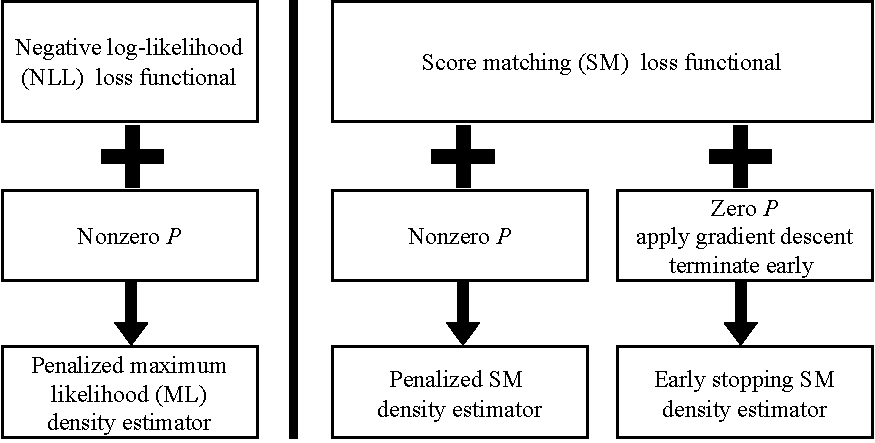
\includegraphics[width=0.7\textwidth]{diagram-loss-pen.pdf}
		\end{figure}
		
%		\begin{itemize}
%		
%			\vspace{5pt}
%			
%			\item Negative log-likelihood (NLL) loss functional: choose a nonzero $P$ $\implies$ penalized maximum likelihood (ML) density estimator
%			
%			\vspace{5pt}
%			
%			\item Score matching (SM) loss functional: 
%			\begin{itemize}
%				\item[--] choose a nonzero $P$ $\implies$ penalized SM density estimator
%				\item[--] choose a zero $P$, use gradient descent algorithm, and terminate the algorithm early $\implies$ early stopping SM density estimator 
%			\end{itemize}
%		\end{itemize}
	\end{itemize}
	
\end{frame}


\begin{frame}{Review of finite-dimensional exponential family}
	
	An $m$-dimensional exponential family 
	% \parencite{Brown1986-ef}
	% denoted by 
	contains all pdfs % of the form 
	\begin{align}
		\tilde{q}_{\theta} \parens{x} := & \, \mu \parens{x} \exp \parens[\big]{ \innerp{\theta}{\varphi \parens{x}}
		% \underbrace{\sum_{j=1}^m \theta_j \varphi_j \parens{x}}_{=: \innerp{\theta}{\varphi \parens{x}}}
		- B \parens{\theta}} \text{ for all } x \in \mathcal{X}, \qquad \theta \in \Theta, 
	\end{align}
	\vspace{-15pt}
	\begin{itemize}
		\item $\mu: \mathcal{X} \to \parens{0, \infty}$ is the \textit{base density}, 
		\item $\theta \in \Theta$ is the \textit{natural parameter}, 
		\item $\varphi: \mathcal{X} \to \mathbb{R}^m$ is the \textit{canonical statistic}, % with $\varphi \parens{x} = \parens{\varphi_1 \parens{x}, \cdots, \varphi_m \parens{x}}^\top$ for all $x \in \mathcal{X}$, 
		\item $B \parens{\theta} := \log \parens[\big]{\int_{\mathcal{X}} \mu \parens{x} \exp \parens{\innerp{\theta}{\varphi \parens{x}}} \mathrm{d} x}$ is the \textit{log-partition function}, and 
		\item $\Theta := \{\theta \in \mathbb{R}^m \bigm| B \parens{\theta} < \infty \}$ is the \textit{natural parameter space}. 
	\end{itemize}
	
	\vspace{10pt}
	
	{\color{defaultcolor}Observations:}
	\begin{itemize}
		\item $\varphi$ maps to an $m$-dimensional space, which can be limited in some applications; 
		\item $\tilde{q}_{\theta}$ depends on $\varphi$ only through its inner product with $\theta$. 
	\end{itemize}
	
%	Let $\varphi: \mathcal{X} \to \mathbb{R}^m$ be a measurable vector-valued function with 
%	\begin{align*}
%		\varphi \parens{x} = \parens{\varphi_1 \parens{x}, \cdots, \varphi_m \parens{x}}^\top, \qquad \text{ for all } x \in \mathcal{X}, 
%	\end{align*}
%	and $\mu: \mathcal{X} \to \parens{0, \infty}$ be a pdf. 
		
% From \eqref{eq-fin-exp-fam}, it is clear that $\log \tilde{q}_{\theta}$, up to an additive constant, is a linear combination of $\log \mu$ and $m$ basis functions $\varphi_1, \cdots, \varphi_m$. 
	
\end{frame}


\begin{frame}{Kernel exponential family $\mathcal{Q}_{\mathrm{ker}}$}
	
	\textit{Kernel exponential family} \parencite{Canu2006-ig}, $\mathcal{Q}_{\mathrm{ker}}$, contains all pdfs % of the form 
	\begin{align}
		q_f \parens{x} := \mu \parens{x} \exp \parens[\big]{ \underbrace{ \innerp{f}{k \parens{x, \,\cdot\,}}_{\mathcal{H}} }_{ = f \parens{x}}
		- A \parens{f}} \text{ for all } x \in \mathcal{X}, \qquad f \in \mathcal{F}, 
	\end{align}
	\vspace{-5pt}
	\begin{itemize}
		\item $k: \mathcal{X} \times \mathcal{X} \to \mathbb{R}$ is the kernel associated with the RKHS $\mathcal{H}$, 
		\item $\innerp{\,\cdot\,}{\,\cdot\,}_{\mathcal{H}}: \mathcal{H} \times \mathcal{H} \to \mathbb{R}$ is the inner product in $\mathcal{H}$, 
		\item $A \parens{f} := \log \parens[\big]{\int_{\mathcal{X}} \mu \parens{x} \exp \parens{f \parens{x} } \mathrm{d} x}$ is the \textit{log-partition functional}, and 
		\item $\mathcal{F} := \{f \in \mathcal{H} \mid A \parens{f} < \infty \}$ is the \textit{natural parameter space}. 
	\end{itemize}
	
%	\vspace{10pt}
%	
%	{\color{defaultcolor} Remark.} $\tilde{q}_{\theta} \in \mathcal{Q}_{\mathrm{fin}}$ can be written in the form of $q_{f} \in \mathcal{Q}_{\mathrm{ker}}$ by choosing $\mathcal{H}$ to be a special finite-dimensional RKHS. 
	
%	\vspace{5pt}
%	
%	Note: 
%	\begin{itemize}
%		\item $f \in \mathcal{F} \subseteq \mathcal{H}$ plays the role of the natural parameter, and 
%		\item $k \parens{x, \,\cdot\,} \in \mathcal{H}$ plays the role of the canonical statistic. 
%	\end{itemize}
			
\end{frame}


%\begin{frame}{Properties of $\calQ_{\mathrm{ker}}$}
%	
%	\begin{itemize}
%		\item If $k$ is bounded, i.e., $\sup_{x \in \calX} \sqrt{k \parens{x, x}} < \infty$, $\mathcal{F} = \mathcal{H}$; 
%		\item $A$ is convex; 
%		\item $A$ is infinitely Fr{\'e}chet differentiable\footnote{{\color{defaultcolor}Definition:} The map $J: \mathcal{H} \to \Real$ is said to be \textit{Fr{\'e}chet differentiable at $f \in \calH$} if there exists a bounded linear operator $\mathrm{D} J \parens{f}: \calH \to \Real$ such that 
%		\begin{align*}
%			\lim_{\substack{\Vert g \Vert_{\calH} \to 0 \\ g \neq 0}} \frac{\vert J \parens{f + g} - J \parens{f} - \mathrm{D} J \parens{f} \parens{g} \vert }{\Vert g \Vert_{\calH}} = 0, 
%		\end{align*} 
%		and $\mathrm{D} J \parens{f}$ is called the \textit{Fr{\'e}chet derivative at $f$}. Higher-order Fr{\'e}chet differentiability and derivatives are defined inductively.}. 
%	\end{itemize}
%	
%\end{frame}


%\begin{frame}{Connection between $\mathcal{Q}_{\mathrm{fin}}$ and $\mathcal{Q}_{\mathrm{ker}}$}
%	
%	Let 
%	\begin{align*}
%		\mathcal{H} = \Bigg\{f \biggm| f := \sum_{j=1}^m \theta_j \varphi_j, \theta_1, \cdots, \theta_m \in \mathbb{R} \Bigg\}
%	\end{align*}
%	and define the inner product between $f = \sum_{j=1}^m \theta_j \varphi_j \in \mathcal{H}$ and $g = \sum_{j=1}^m \eta_j \varphi_j \in \mathcal{H}$ 
%	\begin{align*}
%		\innerp{f}{g}_{\mathcal{H}} := \sum_{j=1}^m \theta_j \eta_j. 
%	\end{align*}
%	Then, $\mathcal{H}$ equipped with $\innerp{\,\cdot\,}{\,\cdot\,}_{\mathcal{H}}$ forms a RKHS. 
%	
%	\vspace{5pt}
%	
%	Under this choice of $\mathcal{H}$, $\mathcal{Q}_{\mathrm{ker}} = \mathcal{Q}_{\mathrm{fin}}$. 
%	
%	\vspace{5pt}
%	
%	If $\mathcal{H}$ is infinite-dimensional, $\mathcal{Q}_{\mathrm{ker}}$ is then a strict generalization of $\mathcal{Q}_{\mathrm{fin}}$. 
%	
%%	whose reproducing kernel is 
%%	\begin{align*}
%%		k \parens{x, y} = \sum_{j=1}^m \varphi_j \parens{x} \varphi_j \parens{y} \text{ for all } x, y \in \mathcal{X}. 
%%	\end{align*}
%	
%\end{frame}


%\begin{frame}{Connection between $\mathcal{Q}_{\mathrm{fin}}$ and $\mathcal{Q}_{\mathrm{ker}}$ (continued)}
%	
%	For $f = \sum_{j=1}^m \theta_j \varphi_j$, 
%	\begin{align*}
%		\innerp{f}{k \parens{x, \,\cdot\,}}_{\mathcal{H}} = \sum_{j=1}^m \theta_j \varphi_j \parens{x} = f \parens{x} = \innerp{\theta}{\varphi \parens{x}}, 
%	\end{align*}
%	and it follows that $q_{f} \parens{x} = \tilde{q}_{\theta} \parens{x}$ for all $x \in \mathcal{X}$. 
%
%	\vspace{10pt}
%	
%	Thus, under this choice of $\mathcal{H}$, $\mathcal{Q}_{\mathrm{ker}} = \mathcal{Q}_{\mathrm{fin}}$. 
%	
%	\vspace{10pt}
%	
%	If $\mathcal{H}$ is infinite-dimensional, $\mathcal{Q}_{\mathrm{ker}}$ is then a strict generalization of $\mathcal{Q}_{\mathrm{fin}}$. 
%
%\end{frame}


\begin{frame}{Assumptions on $\mu$, $\mathcal{H}$, and $k$}
	
	\begin{itemize}
		\item $\mu$ is a continuously differentiable pdf. % supported over $\calX$. 
		
		\vspace{5pt}
		
		\item $\mathcal{H}$ does \emph{not} contain constant functions, which ensures identifiability, i.e., $q_{f_1} = q_{f_2}$ if and only if $f_1 = f_2$. 
		
		\vspace{5pt}
		
		\item $\calH$ is infinite-dimensional. 
		
		\vspace{5pt}
		
		\item $k$ is 
		\begin{itemize}
			\item twice continuously differentiable, which ensures all quantities shown later to be well-defined, and 
			\item bounded, i.e., $\sup_{x \in \mathcal{X}} \sqrt{k \parens{x, x}} < \infty$, which implies $\mathcal{F} = \mathcal{H}$ and makes all optimization problems considered later unconstrained.
		\end{itemize}
		
	\end{itemize}
	
\end{frame}


%\begin{frame}
%	
%	Focus on the nonparametric approaches in the kernel exponential family. 
%	
%	when reviewing the literature, follow the roadmap: method, theory, computation
%	
%	\begin{itemize}
%		\item NLL approach 
%		\begin{itemize}
%			\item with no constraint, no solution 
%			\item regularized approaches
%			\begin{itemize}
%				\item regularize the function space 
%				\item add a penalty term 
%				\item $A$ is hard to deal with --- doubly dual embedding 
%			\end{itemize}
%		\end{itemize}
%		
%		\item SM approach
%		\begin{itemize}
%			\item connection to H-divergence, motivation 
%			\item in kernel exponential family 
%		\end{itemize}
%	\end{itemize}
%	
%\end{frame}


%\begin{frame}{Nonparametric density estimation in $\mathcal{Q}_{\mathrm{ker}}$}
%
%	Minimize 
%	\begin{align*}
%		\widehat{L} \parens{q} + \lambda P \parens{q}, \qquad \text{ subject to } q \in \mathcal{Q}_{\mathrm{ker}}. 
%	\end{align*}
%	
%\end{frame}



\begin{frame}{Minimizing the NLL loss functional}
	
	(Averaged) NLL loss functional 
	\begin{align}
		\widehat{L}_{\NLL} \parens{q} := - \frac{1}{n} \sum_{i=1}^n \log q \parens{X_i}
	\end{align}
	
	With $q = q_f \in \mathcal{Q}_{\mathrm{ker}}$, we can write $\widehat{L}_{\NLL} \parens{q}$ as 
	\begin{align}
		\widehat{J}_{\NLL} \parens{f} := A \parens{f} - \frac{1}{n} \sum_{i=1}^n f \parens{X_i}
	\end{align}
	
	{\color{defaultcolor} Bad News:} Minimizing $\widehat{J}_{\NLL}$ over $\mathcal{H}$ has {\color{red} no solution} \parencite{Fukumizu2009-uu}. 
	
	\vspace{5pt}
	
	{\color{defaultcolor} Remedy:} Impose certain kind of {\color{red} regularization} to obtain a solution. 
	
\end{frame}


%\begin{frame}{Minimize $\widehat{J}_{\NLL}$ over nested finite-dimensional subspaces of $\mathcal{H}$}
%	
%	% Instead of minimizing $\widehat{J}_{\NLL}$ over the entire $\mathcal{H}$, 
%	\textcite{Fukumizu2009-uu} proposed to minimize $\widehat{J}_{\NLL}$ over a series of nested finite- dimensional subspaces of $\mathcal{H}$ that enlarge with the sample size $n$, 
%	\begin{align*}
%		\big\{ \mathcal{H}^{(m_n)} \big\}_{m_n \in \mathbb{N}} \text{ satisfying } \mathcal{H}^{(m_n)} \subset \mathcal{H}^{(m_{n+1})}. 
%	\end{align*}
%	
%	\begin{itemize}
%		\item Established the consistency of his density estimator; % If $p_0 \in \mathcal{Q}_{\ker}$ and $\hat{f}_{\NLL}^{\parens{m_n}} := \argmin_{f \in \mathcal{H}^{\parens{m_n}}} \widehat{J}_{\NLL} \parens{f}$ exists for all $n$, $q_{\hat{f}_{\NLL}^{\parens{m_n}}}$ is consistent for $p_0$ under the KL-divergence; 
%		\vspace{5pt}
%		\item No guidelines on how to construct these $\mathcal{H}^{\parens{m_n}}$; 
%		\vspace{5pt}
%		\item % Even if we know how to construct $\mathcal{H}^{\parens{m_n}}$, 
%		To compute the minimizer in $\mathcal{H}^{\parens{m_n}}$, need to {\color{red} work with $A$ and its derivatives} (involving integration over a possibly high-dimensional space)  --- {\color{red} difficult task!}
%		% need to use an iterative optimization algorithm to compute the minimizer within $\mathcal{H}^{\parens{m_n}}$. 
%		% $\hat{f}_{\NLL}^{\parens{m_n}}$. 
%	\end{itemize}
%	
%\end{frame}


\begin{frame}{Minimizing the penalized NLL loss functional}
	
%	Choose a nonzero $P$ and $\lambda > 0$, and minimize 
%	\begin{align*}
%		\widehat{J}_{\NLL} \parens{f} + \lambda \widetilde{P} \parens{f}, \qquad \text{ subject to } f \in \mathcal{H}, 
%	\end{align*}
%	where 
	
	\textcite{Gu1993-na} proposed to minimize 
	\begin{align}
		\widehat{J}_{\NLL} \parens{f} + \lambda \widetilde{P} \parens{f}, \qquad \text{ subject to } f \in \mathcal{H}. 
	\end{align}
	where $\widetilde{P}: \mathcal{H} \to [0, \infty)$ is $\widetilde{P} \parens{f} := P \parens{q_f}$ for all $f \in \mathcal{H}$. 
	
	\vspace{5pt}
	
	\begin{itemize}
		\item Established the existence and the uniqueness of the minimizer in $\mathcal{H}$; 
		% \item No representer theorem exists; %, as $A$ involves all points in $x \in \mathcal{X}$. 
		\item This minimizer in $\mathcal{H}$ is {\color{red} not} computable. Proposed to minimize over 
		\begin{align*}
			\bigg\{f \Bigm| f := \sum_{i=1}^n \alpha_i k \parens{X_i, \,\cdot\,}, \alpha_1, \cdots, \alpha_n \in \mathbb{R} \bigg\}. 
		\end{align*}
		\textcite{Gu1993-lf} proposed an iterative algorithm to compute the minimizer. \\ 
		
		{\color{red} Main difficulty:} Need to work with {\color{red}$A$ and its derivatives}, which involve integration over a possibly high-dimensional space. 
		
%		\item This minimizer in $\mathcal{H}$ is {\color{red} not} computable. Proposed to minimize over $\calH_0 \oplus \widetilde{\calH}_n$, where $\calH_0 := \{ f \in \calH \mid \widetilde{P} \parens{f} = 0 \}$ and 
%		\begin{align*}
%			\widetilde{\mathcal{H}}_n := \bigg\{f \Bigm| f := \sum_{i=1}^n \alpha_i k \parens{X_i, \,\cdot\,}, \alpha_1, \cdots, \alpha_n \in \mathbb{R} \bigg\}. 
%		\end{align*}
%		\textcite{Gu1993-lf} proposed an iterative algorithm to compute the minimizer. \\ 
%		
%		{\color{red} Main difficulty:} Need to work with {\color{red}$A$ and its derivatives}, which involve integration over a possibly high-dimensional space. 
		
		 % used {\color{red} quadrature rule} to approximate $A$ and its derivatives. 
		 
		% and established the convergence rate of $q_{\tilde{f}_{\NLL}^{\parens{\lambda}}}$ 
		% under the symmetrized KL-divergence
		%\footnote{KL-divergence between pdfs $p, q$ over $\mathcal{X}$ is $\mathrm{KL} \parens{p \Vert q} := \int_{\mathcal{X}} p \parens{x} \log \parens{\frac{p \parens{x}}{q \parens{x}}} \mathrm{d} x$. The symmetrized KL-divergence between $p$ and $q$ is $\mathrm{KL} \parens{p \Vert q} + \mathrm{KL} \parens{q \Vert p}$.}
		% , where $\tilde{f}_{\NLL}^{\parens{\lambda}} := \argmin_{f \in \widetilde{\mathcal{H}}_n} \big\{\widehat{J}_{\NLL} \parens{f} + $ $ \lambda \widetilde{P} \parens{f} \big\}$. 
	\end{itemize}
	
\end{frame}


%\begin{frame}{Minimize penalized NLL loss functional (continued)}
%	
%	\textcite{Gu1993-na} proposed to minimize 
%	\begin{align*}
%		\widehat{J}_{\NLL} \parens{f} + \lambda \widetilde{P} \parens{f}, \qquad \text{ subject to } f \in \widetilde{\mathcal{H}}_n. 
%	\end{align*}
%	
%	\vspace{5pt}
%	
%	\begin{itemize}
%		\item \textcite{Gu1993-lf} proposed an iterative algorithm to compute the minimizer. 
%		\item Used the quadrature rule over a dense mesh to approximate $A$ and its derivatives. 
%		\item All numerical examples in \textcite{Gu1993-lf} are restricted to $d \le 2$. 
%		\item For large $d > 2$, computation would become prohibitively expensive and approximations could be poor. 
%	\end{itemize}
%	
%\end{frame}


%\begin{frame}{\textcite{Dai2018-tp} --- doubly dual embedding}
%	
%	Recognize $A$ has a variational representation 
%	\begin{align*}
%		A \parens{f} = & \, \sup_{p \in \mathcal{P} \cap L^2 \parens{\mathcal{X}}} \bigg\{ \innerp{p}{f}_{L^2 \parens{\mathcal{X}}} - \mathrm{KL} \parens{p \Vert \mu} \bigg\}, && \, \text{ for all } f \in \mathcal{H}, \\ 
%		\mathrm{KL} \parens{p \Vert \mu} = & \, \sup_{g \in \mathcal{H}} \bigg\{ \innerp{p}{g}_{L^2 \parens{\mathcal{X}}} - \int_{\mathcal{X}} e^{g \parens{x}} \mu \parens{x} \mathrm{d} x + 1 \bigg\}, && \, \text{ for all } p \in \mathcal{P} \cap L^2 \parens{\mathcal{X}}. 
%	\end{align*}
%	
%	Plug the preceding two equations into $\widehat{J}_{\NLL} \parens{f} + \lambda \widetilde{P} \parens{f}$ and solve 
%	\begin{align*}
%		\maximize_{p \in \mathcal{P} \cap L^2 \parens{\mathcal{X}}} \ \minimize_{f, g \in \mathcal{H}} \ \bigg\{ & \, - \frac{1}{n} \sum_{i=1}^n f \parens{X_i} + \int_{\mathcal{X}} \parens{f \parens{x} - g \parens{x}} p \parens{x} \mathrm{d} x + \\ 
%		& \qquad \int_{\mathcal{X}} e^{g \parens{x}} \mu \parens{x} \mathrm{d} x + \lambda \widetilde{P} \parens{f} \bigg\}. 
%	\end{align*}
%	
%	Not computationally attractive. 
%	
%\end{frame}


\begin{frame}{Minimizing the SM loss functional}
	
	\begin{align}
		\widehat{L}_{\SM} \parens{q} := \frac{1}{n} \sum_{i=1}^n \sum_{u=1}^d \parens[\Bigg]{\frac{1}{2} \parens[\big]{\partial_u \log q \parens{X_i}}^2 + \partial_u^2 \log q \parens{X_i}}, 
	\end{align}
	where $q: \mathcal{X} \to \parens{0, \infty}$ is a twice continuously differentiable pdf, and 
	\begin{align*}
		\partial_u \log q \parens{x} := \frac{\partial}{\partial w_u} \log q \parens{w} \bigg\vert_{w = x}, \qquad \text{ and } \qquad \partial_u^2 \log q \parens{x} := \frac{\partial^2}{\partial w_u^2} \log q \parens{w} \bigg\vert_{w = x}, 
	\end{align*}
	for all $u = 1, \cdots, d$, and $w := \parens{w_1, \cdots, w_d}^\top \in \mathcal{X}$. 
	
\end{frame}




\begin{frame}{$\widehat{L}_{\SM} \parens{q}$ with $q \in \mathcal{Q}_{\mathrm{ker}}$}
	
	With $q = q_f \in \mathcal{Q}_{\mathrm{ker}}$, $\widehat{L}_{\SM} \parens{q}$ becomes 
	\begin{align}
		\widehat{J}_{\SM} \parens{f} := % & \, \frac{1}{2} \sum_{i=1}^n \sum_{u=1}^d \parens{\partial_u f \parens{X_i}}^2 + \sum_{i=1}^n \sum_{u=1}^d \parens[\big]{\partial_u \log \mu \parens{X_i} \partial_u f \parens{X_i} + \partial_u^2 f \parens{X_i} } \nonumber \\
		% \stackrel{\parens{\star}}{=} & \, 
		\frac{1}{2} \innerp{f}{\widehat{C} f}_{\mathcal{H}} - \innerp{f}{\hat{z}}_{\mathcal{H}}, 
	\end{align}
	where $\widehat{C}: \mathcal{H} \to \mathcal{H}$ is 
	\begin{align*}
		\widehat{C} := \frac{1}{n} \sum_{i=1}^n \sum_{u=1}^d \partial_u k \parens{X_i, \,\cdot\,} \otimes \partial_u k \parens{X_i, \,\cdot\,}, 
	\end{align*}
	with $\widehat{C} f = \frac{1}{n} \sum_{i=1}^n \sum_{u=1}^d \partial_u f \parens{X_i} \partial_u k \parens{X_i, \,\cdot\,}$ for all $f \in \mathcal{H}$, and 
	\begin{align*}
		\hat{z} := - \frac{1}{n} \sum_{i=1}^n \sum_{u=1}^d \parens{\partial_u \log \mu \parens{X_i} \partial_u k \parens{X_i, \,\cdot\,} + \partial_u^2 k \parens{X_i, \,\cdot\,}} \in \mathcal{H}. 
	\end{align*}
	
	With fixed $x \in \mathcal{X}$, $\partial_u^s k \parens{x, y} := \frac{\partial^s}{\partial w_u^s} k \parens{x, y}\big\vert_{w = x}$ for all $y \in \calX$, for $s = 1, 2$. %, and $u = 1, \cdots, d$. 
	
\end{frame}


\begin{frame}{Minimizing $\widehat{J}_{\SM}$ over $\mathcal{H}$ has no solution}
	
	{\color{defaultcolor} Good news:} 
	\begin{itemize}
		\vspace{5pt}
		\item $\widehat{J}_{\SM}$ does {\color{red} not} involve $A$. 
		\vspace{5pt}
		\item Minimizing $\widehat{J}_{\SM}$ over $\mathcal{H}$ is a convex problem, as $\widehat{C}$ is self-adjoint positive (semi-)definite. 
	\end{itemize}
	
	\vspace{10pt}
	
	{\color{defaultcolor} Bad news:} Minimizing $\widehat{J}_{\SM}$ over $\calH$ has {\color{red}no solution}. 
		
%		Suppose $\hat{f}_{\SM} := \argmin_{f \in \mathcal{H}} \widehat{J}_{\SM} \parens{f}$ exists. This $\hat{f}_{\SM}$ must satisfy the linear system 
%		\begin{align*}
%			\widehat{C} \hat{f}_{\SM} = \hat{z}. 
%		\end{align*}
%		But, such an $\hat{f}_{\SM}$ does \textit{not} exist, by noting $\widehat{C}$ is \emph{not} invertible. % \widehat{C} is finite-rank operator, and hence, is compact operator. Any compact operator on an infinite-dimensional space is not invertible. https://math.stackexchange.com/questions/4171733/invertibility-of-compact-operator-on-infinite-dimensional-hilbert-space
	
	\vspace{10pt}
	
	{\color{defaultcolor} Remedy:} Impose certain kind of {\color{red} regularization}. 

\end{frame}


\begin{frame}{Penalized SM density estimator}

	\textcite{Sriperumbudur-density-estimation-inf-exp-family} proposed to minimize
	\begin{align}\label{eq-pen-sm-loss}
		\widehat{J}_{\SM} \parens{f} + \frac{\rho}{2} \Vert f \Vert_{\mathcal{H}}^2, \qquad \text{ subject to } f \in \mathcal{H}, 
	\end{align}
	where $\rho > 0$ is the penalty parameter. This is the {\color{red} Tikhonov regularization}. 
	
	\vspace{10pt}
	
	The minimizer of \eqref{eq-pen-sm-loss} exists and is unique. Using a general representer theorem, 
	\begin{align*}
		\hat{f}_{\SM}^{\parens{\rho}} := & \, \argmin_{f \in \mathcal{H}} \bigg\{\widehat{J}_{\SM} \parens{f} + \frac{\rho}{2} \Vert f \Vert_{\mathcal{H}}^2 \bigg\}  
		= \sum_{i=1}^n \sum_{u=1}^d \alpha_{\parens{i-1}d+u}^{\parens{\rho}} \partial_u k \parens{X_i, \,\cdot\,} + \frac{1}{\rho} \hat{z}, 
	\end{align*}
	where $\parens{\alpha_{1}^{\parens{\rho}}, \cdots, \alpha_{nd}^{\parens{\rho}}}^\top \in \mathbb{R}^{nd}$ can be obtained by solving a linear system. % of $nd$ equations. 
	
\end{frame}


\begin{frame}{Penalized SM density estimator --- comments}

%	\textcite{Sriperumbudur-density-estimation-inf-exp-family} proposed to minimize
%	\begin{align}\label{eq-pen-sm-loss}
%		\widehat{J}_{\SM} \parens{f} + \frac{\rho}{2} \Vert f \Vert_{\mathcal{H}}^2, \qquad \text{ subject to } f \in \mathcal{H}, 
%	\end{align}
%	where $\rho > 0$ is the penalty parameter. This is the Tikhonov regularization. 
	
	\begin{itemize}
		\item No need to work with $A$. 
		% Penalized SM density estimator %$q_{\hat{f}_{\SM}^{\parens{\rho}}}$ 
		% is consistent for $p_0$. % under a wide range of metrics measuring distance between two pdfs. 
		\vspace{5pt}
		\item \textcite{Sriperumbudur-density-estimation-inf-exp-family} empirically showed penalized SM density estimator outperforms kernel density estimator, especially when $d$ is large. 
		\vspace{5pt}
		\item No comparison with the (penalized) ML density estimator was conducted by \textcite{Sriperumbudur-density-estimation-inf-exp-family}. 
%		\vspace{5pt}
%		\item Computing $\hat{f}_{\SM}^{\parens{\rho}}$ 
%		\begin{itemize}
%			\vspace{5pt}
%			\item involves solving a linear system of $nd$ equations in $nd$ variables, and 
%			\vspace{5pt}
%			\item requires elementary operations of order $\mathcal{O} \parens{n^3 d^3}$ --- computationally expensive when $n$ or $d$ is large. 
%		\end{itemize}
	\end{itemize}
	
\end{frame}


\section{Contribution 1: Early Stopping Score Matching Density Estimator}


\begin{frame}{Early stopping regularization}
	
%	Instead of explicitly adding a penalty functional to regularize, we use \textit{early stopping} to regularize. 
%	
%	\vspace{10pt}
	
	\begin{itemize}
		\item \textit{Early stopping} is a form of regularization based on choosing when to terminate an iterative optimization algorithm. 
		
		\vspace{5pt}
		
		\item Often referred to as \textit{implicit} regularization, in contrast to the penalized approach by explicitly adding a penalty term. 
	\end{itemize}
	
\end{frame}


\begin{frame}{Early stopping SM density estimator}
	
	Apply gradient descent algorithm with constant step size to minimizing $\widehat{J}_{\SM}$. 
	
	\vspace{10pt}
	
%	The \textit{Fr{\'e}chet gradient operator} of $\widehat{J}_{\SM}$ is a map from $\mathcal{H}$ to $\mathcal{H}$ and is given by 
%	\begin{align*}
%		\nabla \widehat{J}_{\SM} \parens{f} = \widehat{C} f - \hat{z}, \qquad \text{ for all } f \in \mathcal{H}. 
%	\end{align*}
	
	% \vspace{10pt}
	
	Starting with $\hat{f}_{\SM}^{\parens{0}} = 0 \in \mathcal{H}$, gradient descent iterates are 
	\begin{align*}
		\hat{f}_{\SM}^{\parens{t+1}} %= & \, \hat{f}_{\SM}^{\parens{t}} - \tau \parens{\widehat{C} \hat{f}_{\SM}^{\parens{t}} - \hat{z}} \\ 
		= & \, \sum_{i=1}^n \sum_{u=1}^d \alpha_{\parens{i-1}d + u}^{\parens{t+1}} \partial_u k \parens{X_i, \,\cdot\,} + \parens{t + 1} \tau \hat{z}, \qquad \text{ for all } t = 0, 1, 2, \cdots,  %\in \mathbb{N}_0 := \mathbb{N} \cup \{0\}, 
	\end{align*}
	where $\tau > 0$ is step size, and $\parens{\alpha_1^{\parens{t+1}}, \cdots, \alpha_{nd}^{\parens{t+1}}}^\top \in \mathbb{R}^{nd}$ can be obtained by multiplication and addition of certain matrices. 
	% of size at most $nd \times nd$. 
	
%	\vspace{10pt}
%	
%	{\color{defaultcolor}When to stop in practice:} Use $K$-fold cross-validation. 
	
	% {\color{defaultcolor} Computational advantage:} Time complexities of computing $\hat{f}_{\SM}^{\parens{t}}$ and $\hat{f}_{\SM}^{\parens{\rho}}$ are $\mathcal{O} \parens{n^2d^2}$ and $\mathcal{O} \parens{n^3d^3}$, respectively. 
	
	% Computing $\hat{f}_{\SM}^{\parens{t}}$ for a fixed $t \in \mathbb{N}_0$ requires elementary operations of order $\mathcal{O} \parens{n^2d^2}$, whereas computing $\hat{f}_{\SM}^{\parens{\rho}}$ for a fixed $\rho > 0$ requires elementary operations of order $\mathcal{O} \parens{n^3d^3}$. 
	
\end{frame}


\begin{frame}{Numerical example}
	
	\begin{columns}[c]
	    \begin{column}{.5\textwidth}
	    
			{\color{defaultcolor} Goals:} To illustrate 
			\begin{itemize}
				\item early stopping SM density estimator, and 
				\item its similarity with the penalized SM density estimator. 
			\end{itemize}
			
			\vspace{10pt}
			
			{\color{defaultcolor} Data:} \texttt{waiting} variable in the Old Faithful Geyser dataset, which records 299 time intervals (measured in minutes) between the starts of successive eruptions of the Old Faithful Geyser in Yellowstone National Park August 1st -- 15th, 1985. 
			
		\end{column}
		
	    \begin{column}{.5\textwidth}

			\begin{figure}
				\centering
				\includegraphics[width=0.9\textwidth]{../plots/geyser-waiting-histogram.pdf}
				\caption{Histogram of \texttt{waiting} data with the bin width selected by the Freedman--Diaconis rule.}
				\label{fig-histogram}
			\end{figure}
			
	    \end{column}
	\end{columns}
	
\end{frame}


\begin{frame}{Numerical example (continued)}
	
	\begin{itemize}
		\item $\mathcal{X} = \parens{0, \infty}$; 
		
		\vspace{5pt}
		
		\item The base density $\mu$ is pdf of Gamma distribution. %  with shape and scale parameters being 26 and 3, respectively. 
		
	\end{itemize}
	
	\vspace{-10pt}
	
	\begin{figure}
		\centering
		\includegraphics[width=0.8\textwidth]{../plots/baseden-logbaseden-Gamma-36.0-2.0.pdf}
		\caption{Left panel: $\mu$; right panel: $\log \mu$.}
		\label{fig-base-den-log}
	\end{figure}
	
\end{frame}


\begin{frame}{Numerical example (continued)}
	
	\begin{columns}[c]
	    \begin{column}{.5\textwidth}
	    
			The RKHS $\mathcal{H}$ is the one generated by 
			\begin{align*}
				k \parens{s, t} = \exp \parens[\bigg]{-\frac{\parens{s - t}^2}{2 \sigma^2}}, 
			\end{align*}
			for all $s, t \in \calX$, with $\sigma = 5$. 
			
		\end{column}
		
	    \begin{column}{.5\textwidth}

			\begin{figure}
				\centering
				\includegraphics[width=\textwidth]{../plots/gaussian-kernel.pdf}
				\caption{Gaussian kernel function.}
				\label{fig-base-den-log}
			\end{figure}

			
	    \end{column}
	\end{columns}
	
\end{frame}


\begin{frame}{Penalized and early stopping SM density estimators are very similar}

	\begin{figure}
		\centering
		\includegraphics[width=\textwidth]{../plots/waiting-SM-density-estimates-pen-vs-earlystopping-baseden=Gamma-36.0-2.0-entireRKHS-presentation.pdf}
		\caption{Penalized (first row) and early stopping (second row) SM density estimates of \texttt{waiting} data. Purple circle indicates the location of the isolated observation 108.}
		\label{fig-sm-compare}
	\end{figure}
	
\end{frame}


%\begin{frame}{Penalized and early stopping SM density estimators are very similar}
%	
%	\begin{itemize}
%		\item When very large regularization is imposed (large $\rho$ or small $t$), density estimates are very similar to $\mu$; 
%		\item As $\rho$ decreases or $t$ increases, density estimates become more reasonable and reveal the bimodal feature of data; 
%		\item When very small regularization is imposed (small $\rho$ or large $t$), density estimates contain a bump or spike at the isolated observation 108. 
%	\end{itemize}
%	
%\end{frame}


\section{Contribution 2: Comparison of Regularized Density Estimators}

%\begin{itemize}
%	\item Computation the NLL density estimator
%	\item What is the model specification? 
%	\item figure
%	\item conclusion 
%\end{itemize}
	
\begin{frame}{Goal}

	To compare penalized ML and regularized SM density estimators, and understand their similarities and differences. 
	
\end{frame}


\begin{frame}{Penalized ML density estimator}
	
	Choose $\widetilde{P} \parens{f} = \frac{1}{2} \Vert f \Vert_{\mathcal{H}}^2$ and minimize 
	\begin{align}
		\widehat{J}_{\NLL} \parens{f} + \frac{\lambda}{2} \Vert f \Vert_{\mathcal{H}}^2, \qquad \text{ subject to } f \in \mathcal{H}. 
	\end{align}
	
	{\color{defaultcolor}Good news:} This minimization problem has a unique minimizer in $\mathcal{H}$. 
	
	\vspace{10pt}
	
	{\color{defaultcolor}Bad news:} The representer theorem {\color{red}fails}. This unique minimizer in the infinite- dimensional $\mathcal{H}$ is {\color{red}not} computable. 
	
	\vspace{10pt}
	
	{\color{defaultcolor}Remedy:} Use a finite-dimensional subspace 
	\begin{align}
		\widetilde{\calH} := \bigg\{ f \Bigm| f := \sum_{j=1}^m \beta_j k \parens{w_j, \,\cdot\,}, \beta_1, \cdots, \beta_m \in \mathbb{R} \bigg\}
	\end{align}
	to approximate this minimizer, where $w_1, \cdots, w_m \in \calX$ are pre-specified. 
	%where $m = 180$, and $\parens{w_1, \cdots, w_{180}} = \parens{1, \cdots, 180}$. 
	
\end{frame}


\begin{frame}{Computation of penalized ML density estimator}
	
%	With $w_1, \cdots, w_m \in \mathcal{X}$ pre-specified, we choose the finite-dimensional space to be 
%	\begin{align*}
%		\mathcal{F}_0 := \bigg\{ f \Bigm| f := \sum_{j=1}^m \beta_j k \parens{w_j, \,\cdot\,}, \beta_1, \cdots, \beta_m \in \mathbb{R} \bigg\}. 
%	\end{align*}
	
	With $f = \sum_{j=1}^m \beta_j k \parens{w_j, \,\cdot\,} \in \widetilde{\calH}$, we can write $\widehat{J}_{\NLL} \parens{f} + \frac{\lambda}{2} \Vert f \Vert_{\mathcal{H}}^2$ as 
	\begin{align}
		\widetilde{J}_{\NLL, \lambda} \parens{\bbeta} := \widetilde{A} \parens{\bbeta} - \bbeta^\top \parens[\bigg]{\frac{1}{n} \bK_1 \mathbf{1}_n} + \frac{\lambda}{2} \bbeta^\top \bK_2 \bbeta, 
	\end{align}
	% where 
	\vspace{-10pt}
	\begin{itemize}
		\item $\bbeta := \parens{\beta_1, \cdots, \beta_m}^\top \in \mathbb{R}^m$, 
		\item $\widetilde{A} \parens{\bbeta} := A \parens[\big]{\sum_{j=1}^m \beta_j k \parens{w_j, \,\cdot\,}}$, 
		\item the $\parens{j, i}$-entry of $\bK_1 \in \mathbb{R}^{m \times n}$ is $k \parens{w_j, X_i}$, % for all $i = 1, \cdots, n$, $j = 1, \cdots, m$, 
		\item the $\parens{j, j'}$-entry of $\bK_2 \in \mathbb{R}^{m \times m}$ is $k \parens{w_{j}, w_{j'}}$, % for all $j, j' = 1, \cdots, m$, and 
		\item $\mathbf{1}_n := \parens{1, \cdots, 1}^\top \in \mathbb{R}^n$. 
	\end{itemize}
	
	\vspace{10pt}
	
	Use gradient descent algorithm to compute the minimizer of $\widetilde{J}_{\NLL, \lambda}$ over $\mathbb{R}^m$. 
	
	Approximate $\nabla \widetilde{A} \parens{\bbeta}$ using the Monte Carlo method. 
	
\end{frame}


%\begin{frame}{Computation of penalized ML density estimator (continued)}
%	
%	\begin{itemize}
%		\item With a fixed $\lambda > 0$, use gradient descent algorithm to compute the minimizer of $\widetilde{J}_{\NLL, \lambda}$ over $\mathbb{R}^m$, 
%		\begin{align*}
%			\beta_{\NLL}^{\parens{t+1}} = \beta_{\NLL}^{\parens{t}} - \gamma \parens[\bigg]{\nabla \widetilde{A} \parens{\beta_{\NLL}^{\parens{t}}} - \frac{1}{n} K_1 \mathbf{1}_n + \lambda K_2 \beta_{\NLL}^{\parens{t}}}, \quad \text{ for all } t \in \mathbb{N}_0, 
%		\end{align*}
%		where $\gamma > 0$ is the constant step size. 
%		
%		\vspace{5pt}
%		
%		\item At each iteration, approximate $\nabla \widetilde{A} \parens{\beta}$ using the Monte Carlo method. 
%		
%		\vspace{5pt}
%		
%		\item Terminate the algorithm when 
%		\begin{align*}
%			\big\Vert \nabla \widetilde{J}_{\NLL, \lambda} \parens{\beta_{\NLL}^{\parens{t}}} \big\Vert_2
%		\end{align*}
%		does not exceed a pre-specified tolerance parameter. 
%	\end{itemize}
%	
%\end{frame}


\begin{frame}{Computation of regularized SM density estimators}
	
	For comparability purpose, also compute regularized SM density estimators in $\widetilde{\calH}$. 
	
	\vspace{5pt}
	
	\begin{itemize}
		\item Penalized SM density estimator: with a fixed $\rho > 0$, $\argmin_{f \in \widetilde{\calH}} \big\{\widehat{J}_{\SM} \parens{f} + $ $ \frac{\rho}{2} \Vert f \Vert_{\mathcal{H}}^2 \big\}$ can be obtained by solving a linear system; % of $m$ equations in $m$ variables; 
		
		\vspace{5pt}
		
		\item Early stopping SM density estimator:
		% apply the gradient descent algorithm to minimizing $\widehat{J}_{\SM}$ over $\mathcal{F}_0$. 
		with $\tilde{f}_{\SM}^{\parens{0}} = 0$, gradient descent iterates are 
		\begin{align*}
			\tilde{f}_{\SM}^{\parens{t}} := \sum_{j=1}^m \tilde{\beta}_j^{\parens{t}} k \parens{w_j, \,\cdot\,}, \qquad \text{ for all } t = 0, 1, 2, \cdots, 
		\end{align*}
		where $\parens{\tilde{\beta}_1^{\parens{t}}, \cdots, \tilde{\beta}_m^{\parens{t}}}^\top \in \mathbb{R}^m$ can be obtained by matrix addition and multiplication. % multiplication and addition of certain matrices of size at most $m \times m$. 
	\end{itemize}
	
\end{frame}


\begin{frame}{Numerical example}
	
	Still use \texttt{waiting} data to empirically compare penalized ML and regularized SM density estimators. 
	
	\vspace{5pt}
	
	Choose $\widetilde{\calH}$ to be 
	\begin{align}
		\bigg\{ f \Bigm| f := \sum_{j=1}^m \beta_j k \parens{w_j, \,\cdot\,}, \beta_1, \cdots, \beta_m \in \mathbb{R} \bigg\}, 
	\end{align}
	where $m = 201$, and $\parens{w_1, \cdots, w_{201}} = \parens{1, \cdots, 201}$. 
		
\end{frame}


\begin{frame}{No bump/spike in penalized ML density estimates}
%{Numerical example --- \texttt{waiting} data}
	
	\begin{figure}
		\centering
		\includegraphics[width=0.95\textwidth]{../plots/waiting-ML-vs-SM-density-estimates-baseden=Gamma-36-2-gridpoint=1-202-1-presentation.pdf}
		\caption{Penalized ML (first row), penalized SM (second row), and early stopping SM (third row) density estimates of \texttt{waiting} data. Purple circle indicates the location of isolated observation 108.}
		\label{fig-sm-ml-compare-with108}
	\end{figure}

\end{frame}


%\begin{frame}{Observations}
%	
%	As the amount of regularization becomes smaller ($\lambda$ and $\rho$ become smaller and $t$ becomes larger), 
%	\begin{itemize}
%		\item regularized SM density estimates contain a bump or become a spike at the isolated observation 108, but 
%		\item penalzied ML density estimates do not, even when $\lambda = 0$. 
%	\end{itemize}
%	
%\end{frame}


\begin{frame}{No bump/spike in regularized SM density estimates if 108 is removed}
% {Numerical example without isolated observation 108 --- no bump/spike}
	
	\begin{figure}
		\centering
		\includegraphics[width=0.95\textwidth]{../plots/waiting-ML-vs-SM-density-estimates-baseden=Gamma-36-2-gridpoint=1-202-1-no108-presentation.pdf}
		\caption{Penalized ML (first row), penalized SM (second row), and early stopping SM (third row) density estimates of \texttt{waiting} data with isolated observation 108 removed.}
		\label{fig-sm-ml-compare-no108}
	\end{figure}

\end{frame}


\begin{frame}{Explanation of spike in penalized SM density estimates when $\rho$ is tiny}
	
	The penalized SM density estimator is obtained by minimizing $\widehat{L}_{\SM} \parens{q_f} + \frac{\rho}{2} \Vert f \Vert_{\mathcal{H}}^2$, where, with $d = 1$, 
	\begin{align}
		\widehat{L}_{\SM} \parens{q_f} = & \, \underbrace{\frac{1}{n} \sum_{i \neq i^*} \parens[\bigg]{\frac{1}{2} \parens[\big]{ \parens{\log q_f}' \parens{X_i}}^2 + \parens{\log q_f}'' \parens{X_i}}}_{=: \parens{\mathrm{I}}} + \nonumber \\ 
		& \qquad \qquad \underbrace{\frac{1}{n} \parens[\bigg]{\frac{1}{2} \parens[\big]{ \parens{\log q_f}' \parens{X_{i^*}}}^2 + \parens{\log q_f}'' \parens{X_{i^*}}}}_{=: \parens{\mathrm{II}}}, 
	\end{align}
	and $X_{i^*}$ denotes the isolated observation. 
	
	\vspace{5pt}
	
	When $\rho$ is tiny, we are effectively minimizing $\widehat{L}_{\SM}$ part. 
	
\end{frame}


\begin{frame}{Explanation of spike in penalized SM density estimates when $\rho$ is tiny}
	
	Notice 
	\begin{enumerate}
		\item $\log q_f$ is a linear combination of $\log \mu$ and Gaussian kernel functions, \label{explain-1}
		\item Gaussian kernel functions are local basis functions, and \label{explain-2}
		\item a spike is essentially a local maximum. \label{explain-3}
	\end{enumerate}
	
	\vspace{10pt}
	
	Then, putting a spike in $\log q_f$ at $X_{i^*}$ has the effects of 
	\begin{itemize}
		\item forcing $\parens{\parens{\log q_f}' \parens{X_{i^*}}}^2 \approx 0$ (due to \ref{explain-1} and \ref{explain-3}), 
		\item reducing the value of $\parens{\log q_f}'' \parens{X_{i^*}}$ (due to \ref{explain-1} -- \ref{explain-3}) and that of (II) a lot, 
		\item not affecting $\parens{\mathrm{I}}$ much (due to \ref{explain-2}), and 
		\item reducing the value of $\widehat{L}_{\SM}$ a lot. 
	\end{itemize}
	
\end{frame}


%A similar explanation holds for the early stopping SM density estimator. As we keep running the gradient descent algorithm, we are searching for a $q_f$ that can reduce the value of $\widehat{L}_{\SM}$ as much as possible. With an isolated observation $X_{i^*}$ being present and local basis functions being used, putting a spike at $X_{i^*}$ can achieve this goal. 


\section{Contribution 3: The Sensitivity of Density Estimators via the Influence Function}

%Influence function 
%
%\begin{itemize}
%	\item motivation 
%	\item definition, different versions
%	\item interpretation 
%	\item example
%	\item what can be regarded as robust?
%	\item application 
%\end{itemize}


\begin{frame}{Goals}
	
	% Use the \textit{influence function} to understand the sensitivity of these three density estimators. 
	\begin{enumerate}
		\item To develop a set of tools to understand the sensitivity of density estimators, and 
		\item To understand the sensitivities of penalized ML and SM density estimators\footnote{We drop early stopping SM density estimator as it is very similar to penalized SM density estimator. } in $\mathcal{Q}_{\mathrm{ker}}$ to the presence of an isolated observation. % using the tools developed in the preceding section. 
	\end{enumerate}
	
\end{frame}


%\begin{frame}
%	
%	Using influence function in density estimation 
%	
%	\begin{itemize}
%		\item what is the difficulty? 
%		\item what is the approach to adjust to it? 
%		\item example? --- use figure 
%	\end{itemize}
%	
%\end{frame}


\begin{frame}{Using influence function in density estimation problem}
	
	Influence function \parencite{Hampel1968-gm} was traditionally defined for {\color{red} real- and vector- valued} statistical functionals. 
	
	\vspace{5pt}
	
	The object of main interest in density estimation problem is a pdf. 
	
	\vspace{5pt}
	
	Need to extend the definition of influence function to allow {\color{red} function-valued} statistical functionals. 
	
\end{frame}


\begin{frame}{Influence functions of log-density function evaluated at $x$}

	Let $T$ be a map from the collection of distribution functions over $\calX$ to the class of log-density functions over $\calX$. 
%	\begin{itemize}
%		\item 
%		\item $\widetilde{T}$ be a map from the collection of distributions over $\calX$ to the class of densities over $\calX$. 
%	\end{itemize}
	
	\vspace{10pt}
	
	% Note, if $F$ is a distribution over $\mathcal{X}$, $T \parens{F}$ is a log-density function over $\mathcal{X}$. 
	
	The \textit{influence function of $T \parens{F}$ evaluated at $x \in \calX$} is
	\begin{align}
		\mathrm{IF}_x \parens{T, F, y} := & \, \lim_{\varepsilon \to 0^+} \frac{1}{\varepsilon} \parens[\Big]{ T \parens{ \parens{1 - \varepsilon} F + \varepsilon \delta_y } \parens{x} - T \parens{F} \parens{x} }, % = & \, \frac{\mathrm{d}}{\mathrm{d} \varepsilon} \Big( T \big( (1 - \varepsilon) F + \varepsilon \delta_y \big) (x) \Big) \bigg \vert_{\varepsilon = 0}. 
		%\mathrm{IF}_x \parens{\widetilde{T}, F, y} := & \, \lim_{\varepsilon \to 0^+} \frac{1}{\varepsilon} \parens[\Big]{ \widetilde{T} \parens{ \parens{1 - \varepsilon} F + \varepsilon \delta_y } \parens{x} - \widetilde{T} \parens{F} \parens{x} }, 
	\end{align}
	%respectively, 
	where $\delta_y$ is the point mass 1 at $y \in \calX$. 
	
	\vspace{10pt}
	
	$\mathrm{IF}_x \parens{T, F, y}$
	\begin{itemize}
		\item is the directional derivative of $T$ at $F$ in direction $\delta_y$ evaluated at $x$, and 
		\item measures the effect of an infinitesimal amount of contamination at $y$ on $T \parens{F}$ evaluated at $x$. 
	\end{itemize}
	
\end{frame}


%\begin{frame}{Nature and interpretation of $\mathrm{IF}_x \parens{T, F, y}$}
%	
%	
%	
%	\vspace{10pt}
%	
%	{\color{defaultcolor}Remark.} The nature and interpretation $\mathrm{IF}_x \parens{\widetilde{T}, F, y}$ are similar. 
%	
%\end{frame}


\begin{frame}{Example: normal location model}\label{slide-example}

	\begin{columns}[c]
		\begin{column}{.5\textwidth}
			Let $\calX = \Real$ and $\calQ$ contain all pdfs 
			\begin{align*}
				\tilde{q}_{\theta} \parens{x} := \frac{1}{\sqrt{2 \pi}} \exp \parens[\bigg]{- \frac{\parens{x - \theta}^2}{2}} \text{ for all } x \in \calX, 
			\end{align*}
			where $\theta \in \Real$. 
			
			\vspace{5pt}
			Define $T \parens{F} = \log q_{\theta \parens{F}}$, 
			% and $\widetilde{T} \parens{F} = q_{\theta \parens{F}}$, 
			where 
			\begin{align*}
				q_{\theta \parens{F}} := \argmax_{q_{\theta} \in \calQ} \bigg\{ \int_{\calX} \log q_{\theta} \parens{x} \mathrm{d} F \parens{x} \bigg\}. 
			\end{align*}
			Assume $m_0 := \mathbb{E}_F [X]$ exists. For all $x \in \calX$, 
			\begin{align*}
				\mathrm{IF}_x \parens{T, F, y} = & \, \parens{y - m_0} \parens{x - m_0}. 
				%, \\ \mathrm{IF}_x \parens{\widetilde{T}, F, y} = & \, \frac{1}{\sqrt{2 \pi}} \exp \parens[\bigg]{- \frac{\parens{x - m_0}^2}{2}} \parens{y - m_0} \parens{ x - m_0}. 
			\end{align*}
	\end{column}
	
	\begin{column}{.5\textwidth}
		\begin{figure}
        	\centering
	        \includegraphics[height=0.7\textheight]{../plots/inffunlogden-normal-loc-model-mean=0.0-y=2.0.pdf}
    	    \caption{$\mathrm{IF}_x \parens{T, F, y}$ evaluated at different points with $y = 2$ and $m_0 = 0$. The black dashed vertical line indicates the location of $y$.}
	    \end{figure}
	\end{column}
	\end{columns}
	
\end{frame}


\begin{frame}{Overall influence}

	Fix $y$ and $F$, and view $\mathrm{IF}_x \parens{T, F, y}$
	%and $\mathrm{IF}_x \parens{\widetilde{T}, F, y}$ 
	as a function of $x$. $\mathrm{IF}_x \parens{T, F, y}$
	%and $\mathrm{IF}_x \parens{\widetilde{T}, F, y}$ 
	varies with $x$. 

	\vspace{10pt}
	
	% In other words, with a fixed $F$, a fixed $y$ can have different effects on $T \parens{F} \parens{x}$ for different $x$. 
		
	Define the \textit{overall influence} of $y$ on $T \parens{F}$ 
	%and $\widetilde{T} \parens{F}$ 
	to be 
	\begin{align*}
		\sup_{x \in \mathcal{X}} \big\vert \mathrm{IF}_x \parens{T, F, y} \big\vert, % \qquad \text{ and } \qquad \sup_{x \in \mathcal{X}} \big\vert \mathrm{IF}_x \parens{\widetilde{T}, F, y} \big\vert
	\end{align*}
	which describes the maximal possible effect of $y$ on $T \parens{F}$. % and $\widetilde{T} \parens{F}$, respectively. 
	
	\vspace{25pt}
	
	{\color{defaultcolor}Normal location model example:} 
	\begin{align*}
		\sup_{x \in \calX} \big\vert \mathrm{IF}_x \parens{T, F, y} \big\vert = \begin{cases}
		0, & \, \text{ if } y = m_0 \\ 
		\infty, & \, \text{ otherwise}
		\end{cases}
%		, \qquad 
%		\sup_{x \in \calX} \big\vert \mathrm{IF}_x \parens{\widetilde{T}, F, y} \big\vert = \frac{1}{\sqrt{2 \pi e}} \vert y - m_0 \vert. 
	\end{align*}
	
\end{frame}


%\begin{frame}{Example (continued)}
%	
%	\begin{columns}[c]
%	    \begin{column}{.5\textwidth}
%	    
%			Return to the example on Slide \ref{slide-example}. 
%			
%			\vspace{10pt}
%			
%			Since, for all $x \in \mathbb{R}$, 
%			\begin{align*}
%				\mathrm{IF}_x \parens{T, F, y} = \parens{y - \mathbb{E}_{F} [X]} \parens{ x - \mathbb{E}_F [X]}, 
%			\end{align*}
%			the overall influence of $y$ on $T (F)$ is 
%			\begin{align*}
%				\sup_{x \in \mathbb{R}} \big\vert \mathrm{IF}_x \parens{T, F, y} \big\vert = \begin{cases}
%						0, & \, \text{ if } y = \mathbb{E}_F [X], \\ 
%						\infty, & \, \text{ otherwise}. 
%					\end{cases}
%			\end{align*}
%			
%		\end{column}
%		
%	    \begin{column}{.5\textwidth}
%%	    \begin{figure}
%%	        \centering
%%	        \includegraphics[width=0.9\textwidth]{plots/influence-function-evaluation-example.pdf}
%%	        \caption{Plot of $\mathrm{IF}_x \parens{T, F, y}$ with $y = 1$ and $\mathbb{E}_F [X] = 0$.}
%%	    \end{figure}
%	    \end{column}
%	\end{columns}
%	
%\end{frame}


\begin{frame}{Sample influence function}
	
%	{\color{defaultcolor} Potential issues:} Recall 
%	\begin{align*}
%		\mathrm{IF}_x \parens{T, F, y} := & \, \lim_{\varepsilon \to 0^+} \frac{1}{\varepsilon} \parens[\Big]{ T \parens{ \parens{1 - \varepsilon} F + \varepsilon \delta_y } \parens{x} - T \parens{F} \parens{x} }. % = & \, \frac{\mathrm{d}}{\mathrm{d} \varepsilon} \Big( T \big( (1 - \varepsilon) F + \varepsilon \delta_y \big) (x) \Big) \bigg \vert_{\varepsilon = 0}. 
%		%\mathrm{IF}_x \parens{\widetilde{T}, F, y} := & \, \lim_{\varepsilon \to 0^+} \frac{1}{\varepsilon} \parens[\Big]{ \widetilde{T} \parens{ \parens{1 - \varepsilon} F + \varepsilon \delta_y } \parens{x} - \widetilde{T} \parens{F} \parens{x} }, 
%	\end{align*}
%	The limit by letting $\varepsilon \to 0^+$ may be hard to compute, or $\mathrm{IF}_x \parens{T, F, y}$ may be hard to work with. 
%	
%	\vspace{10pt}
	
	Define the \textit{sample influence function of $T \parens{F_n}$ 
	%and $\widetilde{T} \parens{F_n}$ 
	evaluated at $x \in \mathcal{X}$} to be 
	\begin{align}
		\mathrm{SIF}_{x, \varepsilon} \parens{T, F_n, y} := \frac{1}{\varepsilon} \parens[\Big]{T \parens{\parens{1 - \varepsilon} F_n + \varepsilon \delta_y} \parens{x} - T \parens{F_n} \parens{x}}, %\\ 
		%\mathrm{SIF}_{x, \varepsilon} \parens{\widetilde{T}, F, y} := \frac{1}{\varepsilon} \parens[\Big]{\widetilde{T} \parens[\big]{\parens{1 - \varepsilon} F + \varepsilon \delta_y} \parens{x} - \widetilde{T} \parens{F} \parens{x}}, 
	\end{align}
	%respectively, 
	where $\varepsilon > 0$ and $F_n$ is the empirical distribution function of $X_1, \cdots, X_n$. 
	
	\vspace{10pt}
	
	The corresponding \textit{overall influence} is % $\sup_{x \in \mathcal{X}} \vert \mathrm{SIF}_{x, \varepsilon} \parens{T, F, y} \vert$. 
	\begin{align*}
		\sup_{x \in \mathcal{X}} \vert \mathrm{SIF}_{x, \varepsilon} \parens{T, F, y} \vert. %\qquad \text{ and } \qquad \sup_{x \in \mathcal{X}} \vert \mathrm{SIF}_{x, \varepsilon} \parens{\widetilde{T}, F, y} \vert, 
	\end{align*}
	% respectively. 
	
\end{frame}


\begin{frame}{A special sample influence function}

	With $\varepsilon = \varepsilon_0 := \frac{1}{n+1}$, 
	\begin{align*}
		\parens{1 - \varepsilon_0} F_n + \varepsilon_0 \delta_y = F_{n+1}, 
	\end{align*}
	where $F_{n+1}$ is the empirical distribution function of $X_1, \cdots, X_n$ and $y$. 
	
	\vspace{10pt}
	
	Then, 
	\begin{align}
		\mathrm{SIF}_{x, \varepsilon_0} \parens{T, F_n, y} = \parens{n+1} \parens[\Big]{T \parens{F_{n+1}} \parens{x} - T \parens{F_n} \parens{x}}
	\end{align}
	describes how the value of $T \parens{F_n}$ at $x$ is affected by an additional observation $y$. 
	
\end{frame}


\begin{frame}{Notation}
	
	In order to compare the sensitivities of penalized ML and SM density estimators in $\calQ_{\mathrm{ker}}$, %the sensitivity of penalized ML and SM density estimators in $\mathcal{Q}_{\mathrm{ker}}$, 
	define 
	\begin{align*}
		T_{\lambda} (F) = \log q_{f_{\ML, F}^{\parens{\lambda}}}, \qquad \text{ and } \qquad S_{\rho} (F) = \log q_{f_{\mathrm{SM}, F}^{\parens{\rho}}}, 
	\end{align*}
	where 
	\begin{align*}
		f_{\ML, F}^{\parens{\lambda}} := & \, \argmin_{f \in \mathcal{F}} \Bigg\{ A \parens{f} - \int_{\mathcal{X}} f \parens{x} \mathrm{d} F \parens{x} + \frac{\lambda}{2} \Vert f \Vert_{\mathcal{H}}^2 \Bigg\}, \\
		f_{\SM, F}^{\parens{\rho}} := & \, \argmin_{f \in \mathcal{F}} \Bigg\{ \frac{1}{2} \innerp{f}{C_F f}_{\mathcal{H}} - \innerp{f}{z_F}_{\mathcal{H}} + \frac{\rho}{2} \Vert f \Vert_{\mathcal{H}}^2 \Bigg\}, 
	\end{align*}
	and $C_F := \sum_{u=1}^d \int_{\mathcal{X}} \partial_u k \parens{x, \,\cdot\,} \otimes \partial_u k \parens{x, \,\cdot\,} \mathrm{d} F \parens{x}$, and $z_F := - \sum_{u=1}^d \int_{\mathcal{X}} \big( \partial_u^2 k \parens{x, \,\cdot\,} + \partial_u \log \mu \parens{x} \partial_u k \parens{x, \,\cdot\,} \big) \mathrm{d} F \parens{x}$. 

\end{frame}


\begin{frame}{Focus on the sample influence function}
	
	Expressions of $\mathrm{IF}_{x} \parens{T_{\lambda}, F, y}$ and $\mathrm{IF}_x \parens{S_{\rho}, F, y}$ exist but are hard to work with. 
	
	\vspace{5pt}
	
	We focus on the sample influence function with $\varepsilon = \varepsilon_0 := \frac{1}{n+1}$ and compare numerically. 
	
	\vspace{15pt}
	
	{\color{defaultcolor} Setup:}
	
	\begin{itemize}
		\item Use \texttt{waiting} data with the isolated observation 108 removed. 
		\item Use the same $\mathcal{X}$, $\mu$, $k$, and $\widetilde{\calH}$ as before. 
		\item Choose $y = 20, 22, 24, \cdots, 180$. 
		\item Choose 
		\begin{itemize}
			\item $\lambda = 0, e^{-15}, e^{-14.5}, \cdots, e^{0.5}, e^1$, and 
			\item $\rho = e^{-12}, e^{-11.5}, \cdots, e^0$. 
		\end{itemize}
%		\item To ensure comparability, we let $\mathcal{F} = \mathcal{F}_0$, where 
%		\begin{align*}
%			\mathcal{F}_0 := \bigg\{ f \Bigm| f := \sum_{j=1}^m \beta_j k \parens{w_j, \,\cdot\,}, \beta_1, \cdots, \beta_m \in \mathbb{R} \bigg\}, 
%		\end{align*}
%		where $m = 180$, and $\parens{w_1, \cdots, w_{180}} = \parens{1, \cdots, 180}$. 
	\end{itemize}
	
\end{frame}


\begin{frame}{Example}

	Fix $y = 120$ and $\rho = e^{-11}$. [A] and [B] show $S_{\rho} ((1 - \varepsilon_0) F_n + \varepsilon_0 \delta_y)$ and $S_{\rho} (F_n)$, respectively, and [C] shows 
	\begin{align*}
		\mathrm{SIF}_{x, \varepsilon_0} \parens{S_{\rho}, F_n, y} \propto S_{\rho} \parens{ \parens{1 - \varepsilon_0} F_n + \varepsilon_0 \delta_y} \parens{x} - S_{\rho} \parens{F_n} \parens{x}. 
	\end{align*}
	Overall influence of $y = 120$ is $\approx 2315.48$, achieved roughly at $x$ = 120. 
	
	\begin{figure}
		\centering
		\includegraphics[width=0.9\textwidth]{../plots/inffunlogden-logdensity-density-contam-sm-logpenparam=-11.0-data=120.0-gamma-36.0-2.0-presentation-with-mu.pdf}
	\end{figure}
		
\end{frame}


\begin{frame}{Different $y$ locations give different overall influences}
	
		\begin{columns}[c]
	    \begin{column}{.5\textwidth}
	    
	    	% \textbf{\color{Mulberry} Different $y$ values give different overall influences: }
	    	Still fix $\rho = e^{-11}$ and vary $y$: 
	    	\begin{itemize}
	    		\item if $y$ is $< 40$ or $> 100$ (in low-density region), it has a larger overall influence, and 
	    		\item if $y$ is between 40 and 100 (in high-density region), it has a smaller overall influence. 
	    	\end{itemize}
	    	
	    	\vspace{5pt}
	    		    		    	
	    	Need to look at different $y$ values. 
	    	
		\end{column}
		
	    \begin{column}{.5\textwidth}
	    \begin{figure}
	        \centering
	        \includegraphics[width=0.9\textwidth]{../plots/../plots/waiting-SM-overall-empirical-influence-log-density-estimates-baseden=Gamma-36-2-gridpoints=1-202-1-effects-y.pdf}
	        \caption{Overall influence of $y$ on $S_{\rho}$ vs. $y$, with $\rho = e^{-11}$.}
	    \end{figure}
	    \end{column}
	\end{columns}
\end{frame}


\begin{frame}{Different $\rho$ values give different overall influences}

	\begin{columns}[c]
	    \begin{column}{.5\textwidth}
	    
	    	% Different $y$ values give different overall influences. 
	    	
	    	For a fixed $y = 120$, the smaller the penalty parameter value is, the larger the overall influence of $y$ is. 
	    	
	    	\vspace{10pt}
	
			Need to look at different penalty parameter values. 
		
		\end{column}
		
	    \begin{column}{.5\textwidth}
	    \begin{figure}
	        \centering
	        \includegraphics[width=0.88\textwidth]{../plots/waiting-SM-overall-empirical-influence-log-density-estimates-baseden=Gamma-36-2-gridpoints=1-202-1-effects-rho.pdf}
	        \caption{Overall influence of $y = 120$ on $S_{\rho}$ vs. penalty parameter.}
	    \end{figure}
	    \end{column}
	\end{columns}
\end{frame}


\begin{frame}{Plotting penalty parameter on one axis is a {\color{red} bad} idea}

	\begin{columns}[c]
	    \begin{column}{.6\textwidth}
	    
	    	To show effects of different $y$ and different penalty parameter values on overall influence, we can produce a heat map similar to the right. 
	    	
	    	\vspace{10pt}
	    	
	    	Recall our goal is to compare sensitivities of penalized ML and SM density estimators. 
	    	
	    	\vspace{10pt}
	    	
	    	Plotting penalty parameter on one axis is {\color{red} not} conducive to comparison, as $\lambda$ and $\rho$ are on different scales. 
	    	
		\end{column}
		
	    \begin{column}{.4\textwidth}
	    \begin{figure}
	        \centering
	        \includegraphics[width=\textwidth]{../plots/PenSMFin-PenML-geyser-waiting-logdensity-empIF-supnorm-penaltyparameter-heatmap-bw=5.0-Gamma-36-2-gridpoints=1-202-1-logscale.pdf}
	        \caption{Heat map of overall influence on $S_{\rho}$ vs. $y$ and $\rho$. White rugs indicate locations of \texttt{waiting} data.}
	    \end{figure}
	    \end{column}
	\end{columns}
\end{frame}


\begin{frame}{Penalized SM density estimator is more sensitive to $y$}

	\begin{figure}
		\centering
		\includegraphics[width=0.8\textwidth]{../plots/PenSMFin-PenML-geyser-waiting-logdensity-empIF-supnorm-natparamnorm-heatmap-bw=5.0-Gamma-36-2-gridpoints=1-202-1-logscale.pdf}
		\caption{Heat maps of overall influence of $y$ on $T_{\lambda}$ and $S_{\rho}$ vs. $y$ and RKHS norm of the natural parameter under $F_n$. Red vertical line in left panel indicates the case $\lambda = 0$.}
	\end{figure}
	
\end{frame}


\begin{frame}{Penalized SM density estimator is more sensitive to $y$}

	\begin{figure}
		\centering
		\includegraphics[width=0.8\textwidth]{../plots/PenSMFin-PenML-geyser-waiting-logdensity-empIF-supnorm-natparamnorm-heatmap-bw=5.0-Gamma-36-2-gridpoints=1-202-1-logscale-vertical-line.pdf}
		\caption{Heat maps of overall influence of $y$ on $T_{\lambda}$ and $S_{\rho}$ vs. $y$ and RKHS norm of the natural parameter under $F_n$. Red vertical line in left panel indicates the case $\lambda = 0$.}
	\end{figure}
	
\end{frame}


\begin{frame}{Penalized SM density estimator is more sensitive to $y$}

	\begin{figure}
		\centering
		\includegraphics[width=0.8\textwidth]{../plots/PenSMFin-PenML-geyser-waiting-logdensity-empIF-supnorm-natparamnorm-heatmap-bw=5.0-Gamma-36-2-gridpoints=1-202-1-logscale-horizontal-line.pdf}
		\caption{Heat maps of overall influence of $y$ on $T_{\lambda}$ and $S_{\rho}$ vs. $y$ and RKHS norm of the natural parameter under $F_n$. Red vertical line in left panel indicates the case $\lambda = 0$.}
	\end{figure}
	
\end{frame}


%\begin{frame}{Conclusion}
%	
%	When RKHS norm becomes larger ($\lambda$ and $\rho$ become smaller), penalized SM log-density estimator is more sensitive to an additional observation $y$ than penalized ML log-density estimator. 
%		
%\end{frame}


\begin{frame}{Summary}
	
	Regularized SM density estimators 
	\begin{itemize}
		\item are easy to compute (matrix calculation), but 
		\item are very sensitive to the presence of an isolated observation, especially when there is a small amount of regularization. 
	\end{itemize}
	
	\vspace{10pt}
	
	Penalized ML density estimator 
	\begin{itemize}
		\item is hard to compute (mainly because we need to work with $A$ and its derivatives), but 
		\item is {\color{red} not} sensitive to the presence of an isolated observation, even when no penalty is imposed. 
	\end{itemize}
	
	\vspace{10pt}
	
	\begin{center}
		\textbf{\large {\color{defaultcolor} Use regularized SM density estimators \\ with an \underline{appropriate} amount of regularization!}}
	\end{center}
		
\end{frame}


\section{Future Directions}

%\begin{frame}{Main contributions of the dissertation}
%	
%	\begin{itemize}
%		\item Proposed the early stopping SM density estimator and studied its statistical properties; 
%		\item Numerically compared the regularized SM and ML density estimators; 
%		\item Extended the classic influence function to the density estimation problem; 
%		\item Numerically compared the sensitivities of penalized SM and ML density estimators. 
%	\end{itemize}
%	
%\end{frame}


\begin{frame}{Sensitivity of regularized SM density estimators in higher dimensions}
	
	All numerical examples provided here are restricted to $d = 1$. 
	
	\vspace{10pt}
	
	{\color{defaultcolor} Conjecture:} Regularized SM density estimators in higher dimensions ($d \ge 2$) are also very sensitive to isolated observations when the regularization is small. 
	
	\vspace{10pt}
		
	Need numerical examples to confirm this. 

\end{frame}


%\begin{frame}{Sensitivity of SM estimators in other estimation problems}
%	
%	SM loss functional has been used in studying Gaussian graphical models \parencite{Forbes2015-pe}. 
%	
%	Do {\color{red} not} expect sensitivity issue occurs in this estimation problem, as the canonical statistics are not local basis functions. 
%	
%	\vspace{10pt}
%	
%	Interesting to see whether the applications of the SM loss functional in other types of graphical models result in sensitivity issues. 
%	
%\end{frame}


\begin{frame}{Sensitivity issues when generalized SM loss functional is used}
	
	Several generalized SM loss functionals have been proposed \parencite{Parry2012-pa, Yu2020-fb}. 
	
	\vspace{10pt}
	
	Interesting to 
	\begin{itemize}
		\item apply these generalized SM loss functionals to density estimation problem in $\mathcal{Q}_{\ker}$, and 
		\item investigate the sensitivity issue of the resulting density estimators. 
	\end{itemize}
	% We conjecture, with an appropriate choice of $h$ in \eqref{eq-yu-hdiv}, the resulting density estimators may not be very sensitive to isolated observations. 
	
\end{frame}


\begin{frame}
	
	\begin{center}
		\textbf{\Huge {\color{defaultcolor} Questions?}}
	\end{center}
	
\end{frame}


%\begin{frame}{Using SM loss functional in log-concave density estimation problem}
%	
%	\begin{columns}[c]
%	    \begin{column}{.5\textwidth}
%	    
%			Log-concave density estimation
%	    	\begin{align*}
%	    		\minimize_{q \in \mathcal{Q}_{\mathrm{lc}}} \ \widehat{L} \parens{q} + \lambda P \parens{q}, 
%	    	\end{align*}
%			where $\mathcal{Q}_{\mathrm{lc}}$ is the class of log-concave pdfs over $\mathbb{R}^d$ \parencite{Samworth2018-bw}. 
%	    	
%	    	Dominant approach is to choose $\widehat{L}$ to be the NLL loss functional and zero $P$. 
%	    	
%	    	\vspace{10pt}
%	    	
%	    	Can we choose $\widehat{L}$ to be the SM loss functional? 
%	    	
%		\end{column}
%		
%	    \begin{column}{.5\textwidth}
%	    \begin{figure}
%	        \centering
%	        \includegraphics[width=0.9\textwidth]{../plots/log-concave-density-estimate-mle-with-true.pdf}
%	        \caption{ML log-concave density estimate using 100 random samples from $\mathrm{Normal}(0, 1)$ and true pdf.}
%	    \end{figure}
%	    \end{column}
%	\end{columns}
%\end{frame}

%\appendix
%
%\begin{frame}
%
%	\begin{center}
%		\LARGE{\color{defaultcolor} Appendix}
%	\end{center}
%	
%\end{frame}
%
%\begin{frame}{A review of influence function}
%	
%	Let $F$ be a distribution over $\mathcal{X}$ and $T$ to be a real-valued statistical functional. 
%	
%	\vspace{5pt}
%	
%	The \textit{influence function} of $T$ at $F$ is 
%	\begin{align*}
%		\mathrm{IF} \parens{T, F, y} := & \, \lim_{\varepsilon \to 0^+} \frac{1}{\varepsilon} \parens[\Big]{T \parens[\big]{\parens{1 - \varepsilon} F + \varepsilon \delta_y} - T \parens{F}} \\ 
%		= & \, \frac{\mathrm{d}}{\mathrm{d} \varepsilon} \Big( T \big( (1 - \varepsilon) F + \varepsilon \delta_y \big) \Big) \bigg \vert_{\varepsilon = 0}, 
%	\end{align*} 
%	where $\delta_y$ is the point mass 1 at $y \in \mathcal{X}$. 
%	
%	\vspace{10pt}
%	
%	$\mathrm{IF} \parens{T, F, y}$ 
%	\begin{itemize}
%		\item is the directional derivative of $T$ at $F$ in the direction of $\delta_y$, and 
%		\item measures the effect of an infinitesimally small amount of contamination at $y$ on $T \parens{F}$. 
%	\end{itemize}
%		
%\end{frame}
%
%
%\begin{frame}{Sample influence function}
%	
%	The \textit{sample influence function} of $T$ at $F$ is 
%	\begin{align*}
%		\mathrm{SIF}_{\varepsilon} (T, F, y) := \frac{1}{\varepsilon} \Big( T \big( (1 - \varepsilon) F + \varepsilon \delta_y \big) - T (F) \Big). 
%	\end{align*}
%	$\mathrm{SIF}_{\varepsilon} \parens{T, F, y}$ is a finite-difference approximation of $\mathrm{IF} \parens{T, F, y}$. 
%	
%	\vspace{10pt}
%	
%	\begin{block}{Example: Tukey's sensitivity curve}\vspace{-15pt}
%		\begin{align*}
%			\mathrm{SIF}_{\frac{1}{n+1}} (T, F_n, y)
%		\end{align*}
%		Assess the sensitivity of an estimator to the position of an additional observation $y$ not present in the sample. 
%	\end{block}
%	
%\end{frame}
%
%
%\begin{frame}{Applications of the influence function}
%	
%	\begin{itemize}
%		\item Understand robustness properties of various estimators \parencite{Hampel1986-ig}. 
%		\item Design new estimators with certain desired robustness properties \parencite{Hampel1986-ig}. 
%		\item Identify influential observations in model fitting \parencite{Cook1980-gl}. 
%		\item Perform model validation and selection \parencite{Koh2017-yb}. 
%		\item Design efficient subsampling algorithms to reduce computational burden in training ML and DL models \parencite{Ting2018-fa}. 
%	\end{itemize}
%	
%\end{frame}


%\begin{frame}[allowframebreaks]{Bibliography}
\begin{frame}{Bibliography}
	\renewcommand*{\bibfont}{\tiny}
	\printbibliography

\end{frame}

\begin{frame}{Genesis of $\widehat{L}_{\SM}$}

	$\widehat{L}_{\SM}$ comes from the \textit{Hyv{\"a}rinen divergence} \parencite{Hyvarinen2005-wp}
	\begin{align}
		\mathrm{H} \parens{p_0 \Vert q} := \frac{1}{2} \int_{\mathcal{X}} p_0 \parens{x} \big\Vert \nabla \log p_0 \parens{x} - \nabla \log q \parens{x} \big\Vert_2^2 \mathrm{d} x. 
	\end{align}
	% where $p$ and $q$ are twice continuously differentiable pdfs over $\mathcal{X}$. % and satisfy $\int_{\mathcal{X}} p \parens{x} \Vert \nabla \log p \parens{x} \Vert_2^2 \mathrm{d} x < \infty$ and $\int_{\mathcal{X}} p \parens{x} \Vert \nabla \log q \parens{x} \Vert_2^2 \mathrm{d} x < \infty$. 
	
	\vspace{10pt}
	
	% Assume $p_0 \parens{x} \partial_u \log q \parens{x} \to 0$ as $x \to $ boundary of $\mathcal{X}$ for all $u = 1, \cdots, d$, 
	Under certain regularity conditions, using integration by parts, 
	\begin{align}
		\mathrm{H} \parens{p_0 \Vert q} 
		= & \, \sum_{u=1}^d \int_{\mathcal{X}} p_0 \parens{x} \Bigg[ \frac{1}{2} \parens[\big]{\partial_u \log q \parens{x}}^2 + \partial_u^2 \log q \parens{x} \Bigg] \mathrm{d} x + \text{const}. % \\ & \qquad + \frac{1}{2} \sum_{u=1}^d \int_{\mathcal{X}} p_0 \parens{x} \parens[\big]{\partial_u \log p_0 \parens{x}}^2 \mathrm{d} x, 
	\end{align}
	
	$\widehat{L}_{\SM}$ is the empirical counterpart of $\mathrm{H} \parens{p_0 \Vert q}$ with const omitted. 
	
\end{frame}


\begin{frame}{$\mathrm{IF}_x \parens{T, F, y}$ and $\mathrm{SIF}_{x, \varepsilon} \parens{T, F, y}$ do {\color{red} not} depend on $\mu \parens{x}$}
	
	Let $G$ be a distribution function over $\mathcal{X}$. 
	
	\vspace{10pt}
	
	Suppose $T \parens{G} = \log q_{f_G}$, where $q_{f_G} \in \mathcal{Q}_{\mathrm{ker}}$ for some $f_G \in \mathcal{H}$. Then, 
	\begin{align*}
		& \, T ( (1 - \varepsilon) G + \varepsilon \delta_y ) (x) - T (G) (x) \\ 
		= & \, \big[ \cancel{\log \mu (x)} + f_{(1 - \varepsilon) G + \varepsilon \delta_y} (x) - A (f_{(1 - \varepsilon) G + \varepsilon \delta_y}) \big] \\ 
		& \qquad - \big[ \cancel{\log \mu (x)} + f_{G} (x) - A (f_{G}) \big] \\
		= & \, \big[ f_{(1 - \varepsilon) G + \varepsilon \delta_y} (x) - A (f_{(1 - \varepsilon) G + \varepsilon \delta_y}) \big] - \big[ f_{G} (x) - A (f_{G}) \big]. 
	\end{align*}
	
	\vspace{10pt}
	
	Hence, $\mathrm{IF}_x (T, F, y)$ and $\mathrm{SIF}_{x, \varepsilon} (T, F, y)$ do {\color{red} not} depend on $\mu (x)$, but only on natural parameter part. 
	
\end{frame}


%----------------------------------------------------------------------------------------

\end{document}